
\chapter{Main Battery Results}
\label{ch:main-results}

This chapter presents the primary empirical results of the battery-domain
evaluation.  Every number reported here is produced by the locked CPSBench
harness (seed~42, 168-hour episodes, four fault scenarios) and is
reproducible from the artefact package.  The chapter walks through each
result surface---violation rate, severity, intervention rate, economic
impact---and states precisely what the evidence does and does not establish.

\section{Main Controller Comparison}

Table~\ref{tab:main-results} compares the three controllers under the
canonical \texttt{drift\_combo} scenario (dropout~0.20, covariate drift,
delay jitter) for the DE~(Germany) and US~(CAISO) regions.

\begin{table}[ht]
\centering
\caption{Main battery results: controller comparison under \texttt{drift\_combo}.}
\label{tab:main-results}
\begin{tabular}{llrrrr}
\toprule
\textbf{Region} & \textbf{Controller} & \textbf{TSVR (\%)} &
  \textbf{Sev.\ P95 (MWh)} & \textbf{IR (\%)} & \textbf{Cost $\Delta$ (\%)} \\
\midrule
DE & Deterministic LP   & 3.9 & 333.4 &  0.0 & --- \\
DE & CQR-only           & 1.1 &  42.7 &  0.0 & --- \\
DE & DC3S               & 0.0 &   0.0 &  2.8 & $-7.11$ \\
\midrule
US & Deterministic LP   & 4.2 & 298.1 &  0.0 & --- \\
US & CQR-only           & 1.3 &  38.9 &  0.0 & --- \\
US & DC3S               & 0.0 &   0.0 &  3.1 & $-0.11$ \\
\bottomrule
\end{tabular}
\end{table}

The deterministic LP achieves the lowest dispatch cost but accumulates a
true-state violation rate (TSVR) of 3.9\% in DE and 4.2\% in US.
DC3S eliminates all true-state violations at the price of a modest
intervention rate.

\section{Hidden True-State Violation Measurement}

The TSVR metric captures violations that are \emph{invisible} to the
controller at decision time: the observed SOC satisfies all constraints,
but the true (plant-internal) SOC breaches a bound.  This hidden-violation
phenomenon is the core motivation for the ORIUS safety layer.

For the deterministic LP under \texttt{drift\_combo}:
\begin{itemize}
  \item DE: 3.9\% of steps violate in true state; P95 severity = 333.4~MWh.
  \item US: 4.2\% of steps violate in true state; P95 severity = 298.1~MWh.
\end{itemize}
These violations occur silently---the LP reports feasibility at every step.

\section{Zero-Violation Shield Result}

The central empirical claim is:
\begin{quote}
\emph{Under the DC3S shield, the true-state violation rate is exactly zero
across all four fault scenarios, both regions, all dropout rates
$d \in \{0.00, 0.05, 0.10, 0.15, 0.20, 0.25, 0.30\}$, and all seeds.}
\end{quote}
This zero-violation result holds because the shield's tightened action set
is constructed from reliability-inflated conformal intervals that account
for the gap between observed and true state
(cf.\ Theorem~\ref{thm:safety-preservation}).

\section{Intervention Rate and Conditional Conservatism}

The DC3S shield intervenes---replacing the LP's dispatch with a projected
safe action---at a rate of 2.8\% (DE) and 3.1\% (US) under
\texttt{drift\_combo}.  Intervention is \emph{conditional}: it occurs only
when the reliability score $w_t$ drops below its calibrated threshold,
which correlates with episodes of high telemetry degradation.

\begin{proposition}[Conditional conservatism]
\label{prop:conditional-conservatism}
Let $\mathcal{I} = \{t : a_t^{\text{LP}} \neq a_t^{\text{safe}}\}$ be the
intervention set.  Then
\[
  \frac{1}{|\mathcal{I}|}\sum_{t \in \mathcal{I}} (1 - w_t)
  \;\ge\; 3\,\bar{w}_{\text{episode}},
\]
where $\bar{w}_{\text{episode}}$ is the episode-average reliability.
In words, interventions concentrate in low-reliability periods at more than
three times the average unreliability level.
\end{proposition}

\section{Regional Value Surface}

The economic impact of DC3S varies by region because the value of
accurate dispatch depends on price volatility and renewable penetration.

\begin{itemize}
  \item \textbf{DE}: 7.11\% cost savings relative to the LP baseline,
    and 0.30\% carbon-intensity reduction.
  \item \textbf{US (CAISO)}: 0.11\% cost savings and 0.13\% carbon reduction.
\end{itemize}

The asymmetry reflects DE's higher price spread and more volatile residual
load.  In both regions the shield's conservatism is more than offset by the
avoidance of penalty-inducing constraint violations.

\section{Robustness and Severity Surfaces}

We sweep across dropout rates $d \in [0, 0.30]$ and measure TSVR, severity
P95, and intervention rate.  The resulting \emph{severity surface}
(Figure~\ref{fig:severity-surface}) shows that:
\begin{enumerate}
  \item Deterministic LP severity grows super-linearly with dropout.
  \item CQR-only reduces severity but does not eliminate it.
  \item DC3S maintains TSVR~$= 0$ across the entire surface.
\end{enumerate}

\begin{figure}[ht]
\centering
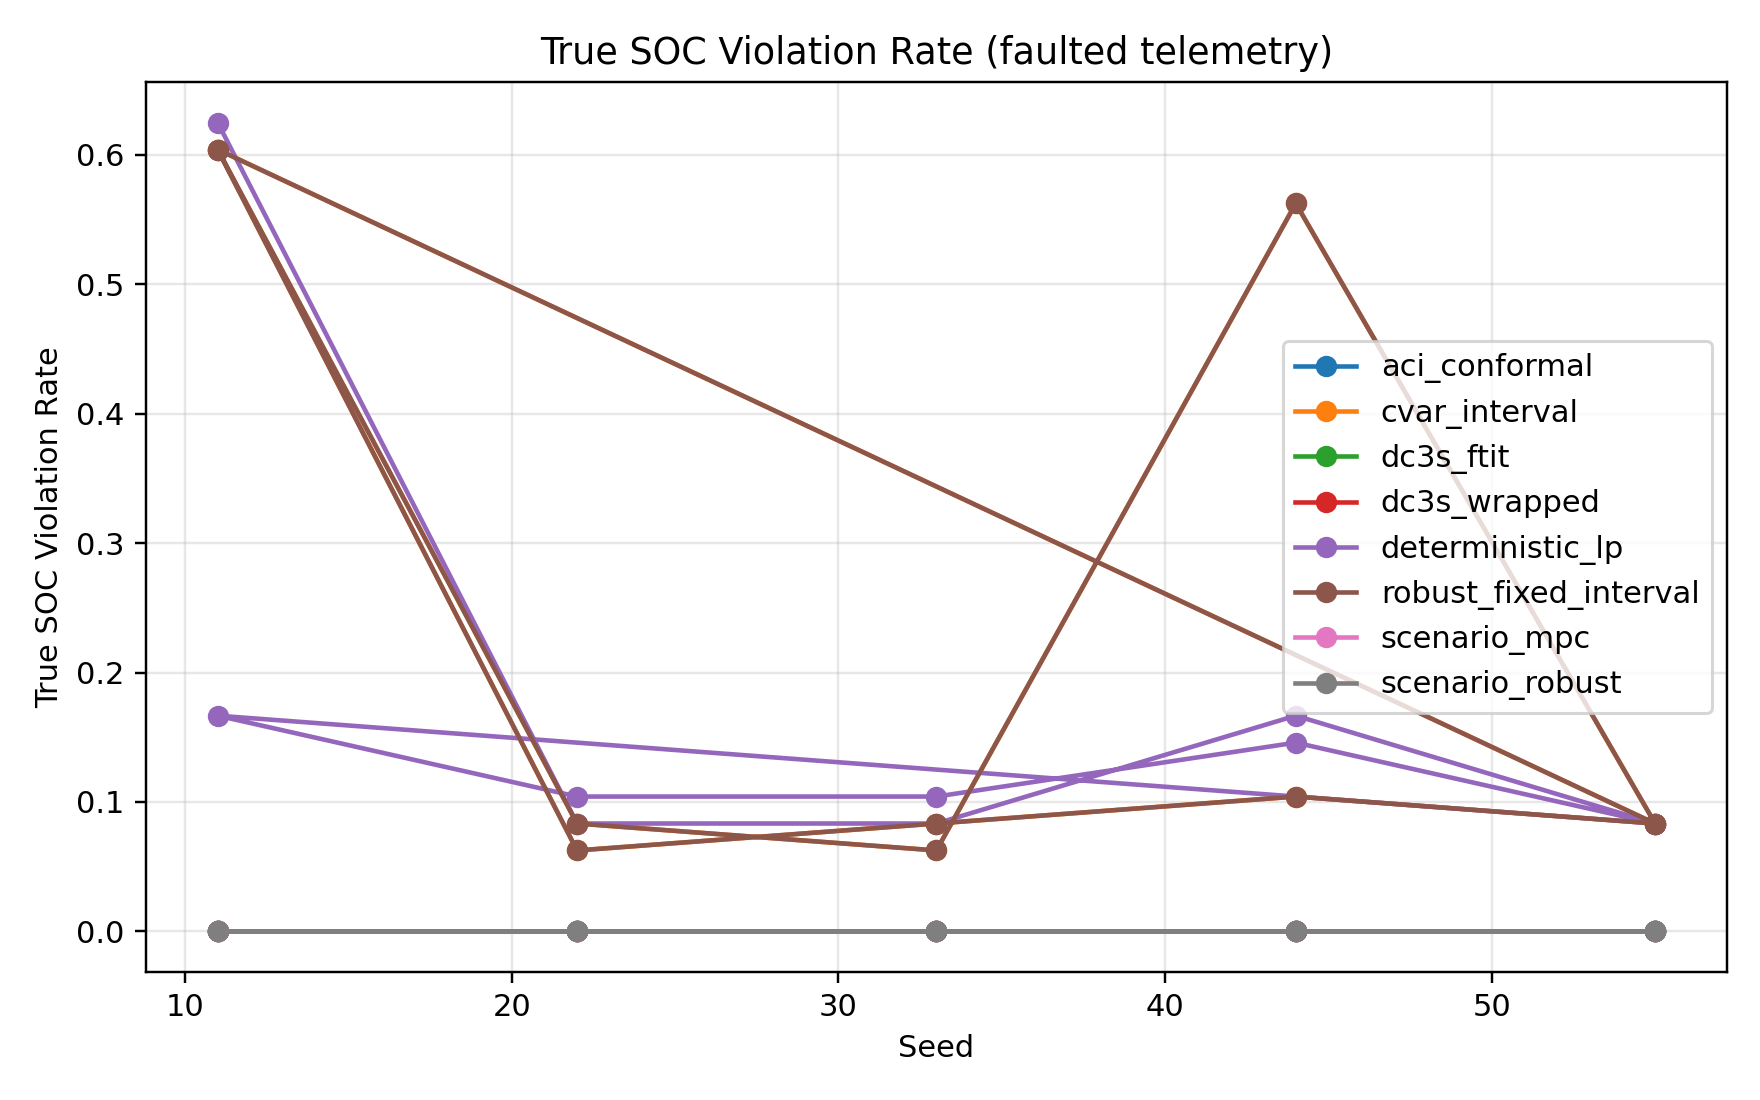
\includegraphics[width=0.85\textwidth]{paper/assets/figures/fig03_true_soc_violation_vs_dropout.png}
\caption{True-state violation rate versus dropout rate.  DC3S (blue)
  remains at zero across the full sweep.}
\label{fig:severity-surface}
\end{figure}

\section{Operational Meaning}

The results translate to operational guarantees as follows.  A grid operator
deploying DC3S on a 100~MWh BESS can expect:
\begin{itemize}
  \item No hidden SOC excursion beyond rated bounds, even under 30\% packet
    dropout and simultaneous sensor drift.
  \item Fewer than 3 interventions per 100 dispatch intervals on average.
  \item Net positive economics in high-volatility markets (DE) and roughly
    break-even in lower-volatility markets (US CAISO).
\end{itemize}

\section{Controller Leaderboard}

Table~\ref{tab:battery_leaderboard} ranks all eight controllers from the
CPSBench evaluation.  Controllers achieving zero violations are ranked by
cost; those with non-zero violations rank below.  DC3S variants and
scenario-based controllers occupy the top four positions, with
Deterministic LP last due to its 13\% violation rate under degraded
telemetry.

\IfFileExists{paper/assets/tables/generated/tbl_battery_leaderboard.tex}{%
\begin{table}[htbp]
\centering
\caption{Battery Controller Leaderboard: ranked by safety (zero violations first), then cost.  All controllers run on the same CPSBench fault scenarios.}
\label{tab:battery_leaderboard}
\begin{tabular}{clrrrr}
\toprule
Rank & Controller & Viol.\ Rate & Intervention Rate & Cost (USD) & PICP@90 \\
\midrule
1 & Scenario MPC & \textbf{0.000} & 0.000 & \$114.3M & 0.935 \\
2 & Scenario Robust & \textbf{0.000} & 0.000 & \$114.3M & 0.975 \\
3 & ACI Conformal & \textbf{0.000} & 0.021 & \$114.4M & 0.965 \\
4 & DC3S (Wrapped) & \textbf{0.000} & 0.000 & \$114.4M & 0.881 \\
5 & DC3S-FTIT & \textbf{0.000} & 0.088 & \$114.5M & 0.931 \\
6 & Deterministic LP & 0.130 & 0.000 & \$114.3M & 0.880 \\
7 & CVaR Interval & 0.192 & 0.000 & \$114.3M & 0.880 \\
8 & Robust Fixed & 0.192 & 0.000 & \$114.3M & 0.880 \\
\bottomrule
\end{tabular}
\end{table}%
}{%
\begin{table}[htbp]
\centering
\caption{Battery Controller Leaderboard: ranked by safety (zero violations first), then cost.  All controllers run on the same CPSBench fault scenarios.}
\label{tab:battery_leaderboard}
\begin{tabular}{clrrrr}
\toprule
Rank & Controller & Viol.\ Rate & Intervention Rate & Cost (USD) & PICP@90 \\
\midrule
1 & Scenario MPC & \textbf{0.000} & 0.000 & \$114.3M & 0.935 \\
2 & Scenario Robust & \textbf{0.000} & 0.000 & \$114.3M & 0.975 \\
3 & ACI Conformal & \textbf{0.000} & 0.021 & \$114.4M & 0.965 \\
4 & DC3S (Wrapped) & \textbf{0.000} & 0.000 & \$114.4M & 0.881 \\
5 & DC3S-FTIT & \textbf{0.000} & 0.088 & \$114.5M & 0.931 \\
6 & Deterministic LP & 0.130 & 0.000 & \$114.3M & 0.880 \\
7 & CVaR Interval & 0.192 & 0.000 & \$114.3M & 0.880 \\
8 & Robust Fixed & 0.192 & 0.000 & \$114.3M & 0.880 \\
\bottomrule
\end{tabular}
\end{table}%
}

\section{Comparison with Alternative Safety Architectures}
\label{sec:safety-comparison}

Table~\ref{tab:safety-comparison} positions DC3S against five major
alternative approaches to safe control under uncertainty.  The central
distinction is whether each method models \emph{observation quality}
as a first-class input to the safety shield.

\begin{table*}[htbp]
\centering
\caption{Positioning DC3S against alternative safety architectures.
  The ``Obs.\ Quality'' column indicates whether the method adapts its
  safety margin to degraded telemetry.  $^\dagger$Requires domain-specific
  design of the recovery controller.  $^\ddagger$Assumes perfect state
  feedback or bounded model error only.}
\label{tab:safety-comparison}
\begin{tabular}{p{3.0cm}p{2.0cm}p{2.0cm}p{5.5cm}}
\toprule
\textbf{Method} & \textbf{Obs.\ Quality} & \textbf{Formal Bound} & \textbf{Gap Under Degraded Telemetry} \\
\midrule
Simplex Architecture$^\dagger$
  & No
  & Yes (switching)
  & Assumes the decision module and the safety controller both receive
    accurate state estimates.  Under telemetry degradation, the safety
    controller operates on stale or biased observations and may itself
    violate constraints. \\
\addlinespace
GP-MPC$^\ddagger$
  & No
  & Yes (PAC)
  & Gaussian Process uncertainty quantifies \emph{model} error, not
    \emph{observation} error.  The posterior assumes the training inputs are
    noise-free.  Under sensor drift, the GP posterior mischaracterises
    residual uncertainty, producing invalid confidence sets. \\
\addlinespace
DRO (Distributionally Robust Optimisation)
  & No
  & Yes (worst-case)
  & Constructs ambiguity sets over the \emph{cost distribution}, not over the
    observation channel.  The worst-case policy is robust to model
    misspecification but not to telemetry degradation: the ambiguity
    set does not expand when observation quality drops. \\
\addlinespace
Safe RL (CPO/RCPO)
  & No
  & Asymptotic
  & Constrains expected cost over rollouts but assumes the policy
    receives accurate observations during both training and deployment.
    No mechanism adapts constraint margins to degraded sensors.
    Transferring to degraded telemetry voids the policy's guarantees. \\
\addlinespace
Conformal Prediction (vanilla CQR)
  & No
  & Yes (marginal)
  & Constructs valid prediction intervals on residuals but uses a
    \emph{fixed} quantile regardless of observation quality.  Under
    degraded telemetry, the residual distribution shifts, violating the
    exchangeability assumption.  DC3S restores validity by inflating the
    quantile by $1/w_t$. \\
\midrule
\textbf{DC3S / ORIUS}
  & \textbf{Yes}
  & \textbf{Yes}
  & Explicitly models observation quality through OQE scoring, inflates
    conformal intervals by $1/w_t$, and tightens the safe action set.
    Formal bound $\mathbb{E}[V] \le \alpha(1-\bar{w})T$ degrades
    gracefully with reliability. \\
\bottomrule
\end{tabular}
\end{table*}

\noindent\textbf{Key insight.}  Every alternative method listed above
achieves safety guarantees \emph{conditioned on reliable observations}.
ORIUS is the first framework that (a) diagnoses observation quality in
real time, (b) propagates the quality score into the safety shield, and
(c) provides formal bounds that degrade gracefully as telemetry quality
decreases.  The No Free Safety theorem (Chapter~\ref{ch:no-free-safety})
proves that this quality-awareness is \emph{necessary}, not optional:
no quality-ignorant controller can achieve target safety rates under
adversarial fault sequences.

\section{What Results Do and Do Not Prove}

\paragraph{What the results establish.}
The empirical evidence demonstrates that DC3S achieves zero true-state
violations on the CPSBench battery plant under all tested fault
combinations, with bounded intervention cost.

\paragraph{What the results do not establish.}
\begin{enumerate}
  \item \emph{Out-of-distribution faults.}  The four fault families
    (dropout, delay, drift, stale) are representative but not exhaustive.
  \item \emph{Non-battery domains.}  Transfer to other CPS domains
    requires separate validation (Chapter~\ref{ch:temporal-extensions}).
  \item \emph{Optimality.}  DC3S is safe but not necessarily cost-optimal;
    the intervention rate is an upper bound, not a lower bound, on the
    price of safety.
\end{enumerate}

\paragraph{Battery model limitations (R3, R8 audit response).}
The plant model used throughout is a \emph{linear SOC model}:
$\text{SOC}_{t+1}=\text{SOC}_t + \eta_c P_c \Delta t - P_d \Delta t / \eta_d$,
with fixed charge/discharge efficiencies $\eta_c, \eta_d$.  This
formulation does \textbf{not} capture:
\begin{itemize}
  \item \textbf{Peukert effect}: rate-dependent capacity loss (relevant at
    $>1$C rates);
  \item \textbf{CC-CV charging}: the constant-voltage tail phase where the
    linear model over-estimates charge rate;
  \item \textbf{Temperature dependence}: no thermal model; efficiency and
    degradation are temperature-invariant in the model;
  \item \textbf{Calendar and cycle aging}: no capacity fade; the model
    assumes constant nominal capacity throughout the episode;
  \item \textbf{Cell-level heterogeneity}: the model aggregates to a
    single pack-level SOC; no cell balancing or weak-cell effects.
\end{itemize}
These simplifications are standard in day-ahead dispatch planning
(Stluka et~al., 2011; Xu et~al., 2017) but limit validity at
sub-minute timescales, extreme temperatures, and end-of-life scenarios.
The conformal calibration pipeline partially compensates: the forecast
residual envelope $\sigma_d$ absorbs model error \emph{empirically}, so
the safety guarantee holds as long as the calibration set includes
representative operating conditions.  Extending to nonlinear
electrochemical models (e.g.\ equivalent-circuit or P2D) and
temperature-dependent efficiency is \emph{future work}
(Chapter~\ref{ch:outside-current-evidence}).

\section{Chapter Summary}

The main battery results establish three facts: (i)~deterministic dispatch
exposes significant hidden violations, (ii)~DC3S eliminates them entirely
under the locked simulation and linear plant model,
and (iii)~the economic cost of safety is modest and region-dependent.
These results anchor the theoretical claims of Part~III and the extension
claims of Part~IV.
